
\documentclass[11pt,a4paper,UTF8]{book}

\usepackage[T1]{fontenc}
\usepackage[utf8]{inputenc}
\usepackage{authblk}

\usepackage{fontspec}                  %引入字体设置宏包
\setmainfont{Times New Roman}             %设置英文正文字体
% Courier New
% Book Antique
\setsansfont{Arial}                    %英文无衬线字体
\setmonofont{Courier New}              %英文等宽字体

\usepackage{ctex} %导入中文包
%\usepackage{ulem}
\usepackage{tocvsec2}
\usepackage{verbatim}

\usepackage{tabularx}
\usepackage{booktabs} 
\usepackage{multirow}
\usepackage{bbding}
\usepackage{float}
\usepackage{xspace}
\usepackage[none]{hyphenat}

\usepackage{graphicx}
\usepackage{subfigure}
\usepackage{pifont}

\usepackage{hyperref}  %制作pdf的目录
\usepackage{subfiles} %使用多文件方式进行

\usepackage{geometry} %设置页边距的包
\geometry{left=2.5cm,right=2cm,top=2.54cm,bottom=2.54cm} %设置书籍的页边距

\usepackage{url}
\hypersetup{hidelinks, %去红框
	colorlinks=true,
	allcolors=black,
	pdfstartview=Fit,
	breaklinks=true
}

% 调整itemlist中的行间距
\usepackage{enumitem}
\setenumerate[1]{itemsep=0pt,partopsep=0pt,parsep=\parskip,topsep=5pt}
\setitemize[1]{itemsep=0pt,partopsep=0pt,parsep=\parskip,topsep=5pt}
\setdescription{itemsep=0pt,partopsep=0pt,parsep=\parskip,topsep=5pt}

% 超链接样式设置
\usepackage{hyperref}
\hypersetup{
	colorlinks=true,
	linkcolor=blue,
	filecolor=blue,
	urlcolor=blue,
	citecolor=cyan,
}

\usepackage{indentfirst}

\usepackage{listings}
\usepackage[usenames,dvipsnames,svgnames, x11names]{xcolor}

\usepackage[most]{tcolorbox}

%展示代码
\definecolor{mygreen}{rgb}{0,0.6,0}
\definecolor{mygray}{rgb}{0.5,0.5,0.5}
\definecolor{mymauve}{rgb}{0.58,0,0.82}
\definecolor{keywordcolor}{rgb}{0.8,0.1,0.5}
\definecolor{webgreen}{rgb}{0,.5,0}
\definecolor{bgcolor}{rgb}{0.92,0.92,0.92}

%定义CMake
\lstdefinelanguage{CMake}
{morekeywords={
		cmake\_minimum\_required,
		project,
		add\_executable,
		add\_library,
		target\_link\_libraries,
		cmake\_parse\_arguments,
		cmake\_language,
		set, unset,
		option,
		string,
		list,
		math,
		message,
		if, elseif, else, endif,
		mark\_as\_advanced,
		foreach, endforeach,
		while, endwhile,
		add\_subdirectory, include, return, include\_gurad,
		function, endfunction,
		macro, endmacro,
		find\_package,
		cmake\_push\_check\_state,
		cmake\_pop\_check\_state,
		cmake\_reset\_check\_state,
		add\_test,
		set\_tests\_properties, 
		check\_c\_source\_runs,
		check\_cxx\_source\_runs,
		check\_fortran\_source\_runs,
		check\_source\_runs,
		check\_compiler\_flag,
		check\_c\_compiler\_flag,
		check\_cxx\_compiler\_flag,
		check\_fortran\_compiler\_flag,
		check\_symbol\_exists,
		check\_cxx\_symbol\_exists,
		check\_linker\_flag,
		cmake\_policy,
		set\_property,
		get\_property,
		define\_property,
		get\_cmake\_property,
		set\_cmake\_property,
		set\_target\_properties,
		get\_target\_property,
		set\_directory\_properties,
		get\_directory\_property,
		set\_source\_files\_properties,
		get\_source\_file\_property,
		set\_tests\_properties,
		get\_tests\_property,
		get\_test\_property,
		cmake\_print\_properties,
		cmake\_print\_variables,
		variable\_watch,
		include\_guard,
		target\_link\_options,
		target\_compile\_definitions,
		target\_compile\_options,
		include\_directories,
		add\_definitions,
		remove\_definitions,
		add\_compile\_definitions,
		add\_compile\_options,
		link\_libraries,
		link\_directories,
		add\_link\_options,
		target\_include\_directories,
		target\_compile\_features,
		add\_custom\_command,
		add\_custom\_target,
		execute\_process,
		cmake\_path,
		get\_filename\_component,
		file,
		configure\_file,
		generate\_export\_header,
		export,
		find\_file,
		find\_library,
		find\_package,
		find\_program,
		pkg\_check\_modules,
		pkg\_search\_module,
		pkg\_get\_variable,
		add\_test,
		enable\_testing,
		set\_tests\_properties,
		site\_name,
		ctest\_empty\_binary\_directory,
		ctest\_start,
		ctest\_configure,
		ctest\_submit,
		ctest\_build,
		ctest\_memcheck,
		ctest\_upload,
		ctest\_test,
		gtest\_add\_tests,
		gtest\_discover\_tests,
		install,
		write\_basic\_package\_version\_file,
		configure\_package\_config\_file,
		cpack\_add\_component,
		cpack\_add\_install\_type,
		cpack\_add\_component\_group,
		ExternalProject\_Add,
		ExternalProject\_Add\_StepDependencies,
		ExternalProject\_Get\_Property,
		ExternalProject\_Add\_Step,
		FetchContent\_Declare,
		FetchContent\_GetProperties,
		FetchContent\_Populate,
		source\_group,
		target\_precompile\_headers,
		qt5\_wrap\_cpp,
		qt5\_wrap\_ui,
		qt5\_add\_resources,
		qt5\_add\_big\_resources,
		qt5\_add\_binary\_resources,
		qt5\_add\_translation,
		qt5\_create\_translation,
		compile\_definitions,
		add\_llvm\_component\_library,
		add\_llvm\_tool,
		llvm\_multisource,
		llvm\_test\_data,
		doxygen\_add\_docs,
	}, %定义关键字
	sensitive=false, %是否大小写敏感
	morecomment=[l]{\#},
	morestring=[b]",
	morestring=[d]',
}

\lstdefinestyle{styleCXX}{
	language = C++,  
	backgroundcolor=\color{blue!3!white}, 
	%basicstyle = \footnotesize,  
	basicstyle      =   \zihao{-5}\ttfamily,
	numberstyle     =   \zihao{-5}\ttfamily,   
	%breakatwhitespace = false,    
	basewidth       =   0.5em,    
	breaklines = true,                 
	captionpos = b,                    
	commentstyle = \color{mygray}\bfseries,
	%extendedchars = false,             
	frame =shadowbox, 
	framerule=0.5pt,
	%frameround = fttt,
	keepspaces=true,
	keywordstyle=\color{blue}\bfseries, % keyword style
	otherkeywords={string}, 
	numbers=left, 
	numbersep=5pt,
	numberstyle=\tiny\color{mygray},
	rulecolor=\color{black},         
	%showspaces=false,  
	%showstringspaces=false, 
	%showtabs=false,    
	%stepnumber=1,         
	stringstyle=\color{mymauve},        % string literal style
	tabsize=2,          
	columns         =   fixed,
	flexiblecolumns,                   
}


\lstdefinestyle{styleCMake}{
	language=CMake,
	backgroundcolor=\color{blue!3!white}, 
	basicstyle=\tt, 
	breakatwhitespace = false,
	breaklines = true,
	captionpos = b,
	commentstyle = \color{mygray}\bfseries, 
	extendedchars =false,             
	frame=shadowbox, 
	tabsize=2,
	framerule=0.5pt,
	keepspaces=true,
	keywordstyle=\color{blue}\bfseries, % keyword style
	otherkeywords={string}, 
	rulecolor=\color{black},
	showspaces=false,
	showstringspaces=false,
	showtabs=false,
	stepnumber=1,
	stringstyle=\color{purple},        % string literal style
}

\lstdefinestyle{stylePython}{
	language        =   Python, % 语言选Python
	backgroundcolor=\color{blue!3!white}, 
	basicstyle      =   \zihao{-5}\ttfamily,
	numberstyle     =   \zihao{-5}\ttfamily,
	keywordstyle    =   \color{blue},
	keywordstyle    =   [2] \color{teal},
	stringstyle     =   \color{magenta},
	commentstyle    =   \color{red}\ttfamily,
	frame = shadowbox, 
	breaklines      =   true,   % 自动换行,建议不要写太长的行
	columns         =   fixed,  % 如果不加这一句,字间距就不固定,很丑,必须加
	basewidth       =   0.5em,
	%basicstyle          =   \sffamily,          % 基本代码风格
	%keywordstyle        =   \bfseries,          % 关键字风格
	%commentstyle        =   \rmfamily\itshape,  % 注释的风格,斜体
	%stringstyle         =   \ttfamily,  % 字符串风格
	flexiblecolumns,                % 别问为什么,加上这个
	%numbers             =   left,   % 行号的位置在左边
	showspaces          =   false,  % 是否显示空格,显示了有点乱,所以不现实了
	numberstyle         =   \zihao{-5}\ttfamily,    % 行号的样式,小五号,tt等宽字体
	showstringspaces    =   false,
	captionpos          =   t,      % 这段代码的名字所呈现的位置,t指的是top上面
	frame               =   lrtb,   % 显示边框
	tabsize=2,  
}

\tcbset{
	commandshell/.style={
		listing only,
		colback=black!75!white,
		colupper=white,
		lowerbox=ignored,
		listing options={
			language={bash},
			basicstyle=\ttfamily,
			columns = fixed,
			flexiblecolumns
		}
}}

\usepackage{tikz}

% URL 正确换行
% https://liam.page/2017/05/17/help-the-url-command-from-hyperref-to-break-at-line-wrapping-point/
\makeatletter
\def\UrlAlphabet{%
	\do\a\do\b\do\c\do\d\do\e\do\f\do\g\do\h\do\i\do\j%
	\do\k\do\l\do\m\do\n\do\o\do\p\do\q\do\r\do\s\do\t%
	\do\u\do\v\do\w\do\x\do\y\do\z\do\A\do\B\do\C\do\D%
	\do\E\do\F\do\G\do\H\do\I\do\J\do\K\do\L\do\M\do\N%
	\do\O\do\P\do\Q\do\R\do\S\do\T\do\U\do\V\do\W\do\X%
	\do\Y\do\Z}
\def\UrlDigits{\do\1\do\2\do\3\do\4\do\5\do\6\do\7\do\8\do\9\do\0}
\g@addto@macro{\UrlBreaks}{\UrlOrds}
\g@addto@macro{\UrlBreaks}{\UrlAlphabet}
\g@addto@macro{\UrlBreaks}{\UrlDigits}
\makeatother

% enable subsubsubsection
% from https://tex.stackexchange.com/questions/274212/correct-hierarchy-levels-of-pdf-bookmarks-for-custom-section-subsubsubsection
\usepackage[depth=3]{bookmark}
\setcounter{secnumdepth}{3}
\setcounter{tocdepth}{4}
\hypersetup{bookmarksdepth=4}

\makeatletter

\newcommand{\toclevel@subsubsubsection}{4}
\newcounter{subsubsubsection}[subsubsection]

\renewcommand{\thesubsubsubsection}{\thesubsubsection.\arabic{subsubsubsection}}

\newcommand{\subsubsubsection}{\@startsection{subsubsubsection}{4}{\z@}%
	{-3.25ex\@plus -1ex \@minus -.2ex}%
	{1.5ex \@plus .2ex}%
	{\normalfont\normalsize\bf\bfseries}}

\newcommand*{\l@subsubsubsection}{\@dottedtocline{4}{11em}{5em}}  

\newcommand{\subsubsubsectionmark}[1]{}
\makeatother

\begin{document}
\begin{sloppypar} %latex中一行文字出现溢出问题的解决方法
	%\maketitle
	
	\begin{center}
		\thispagestyle{empty}
		%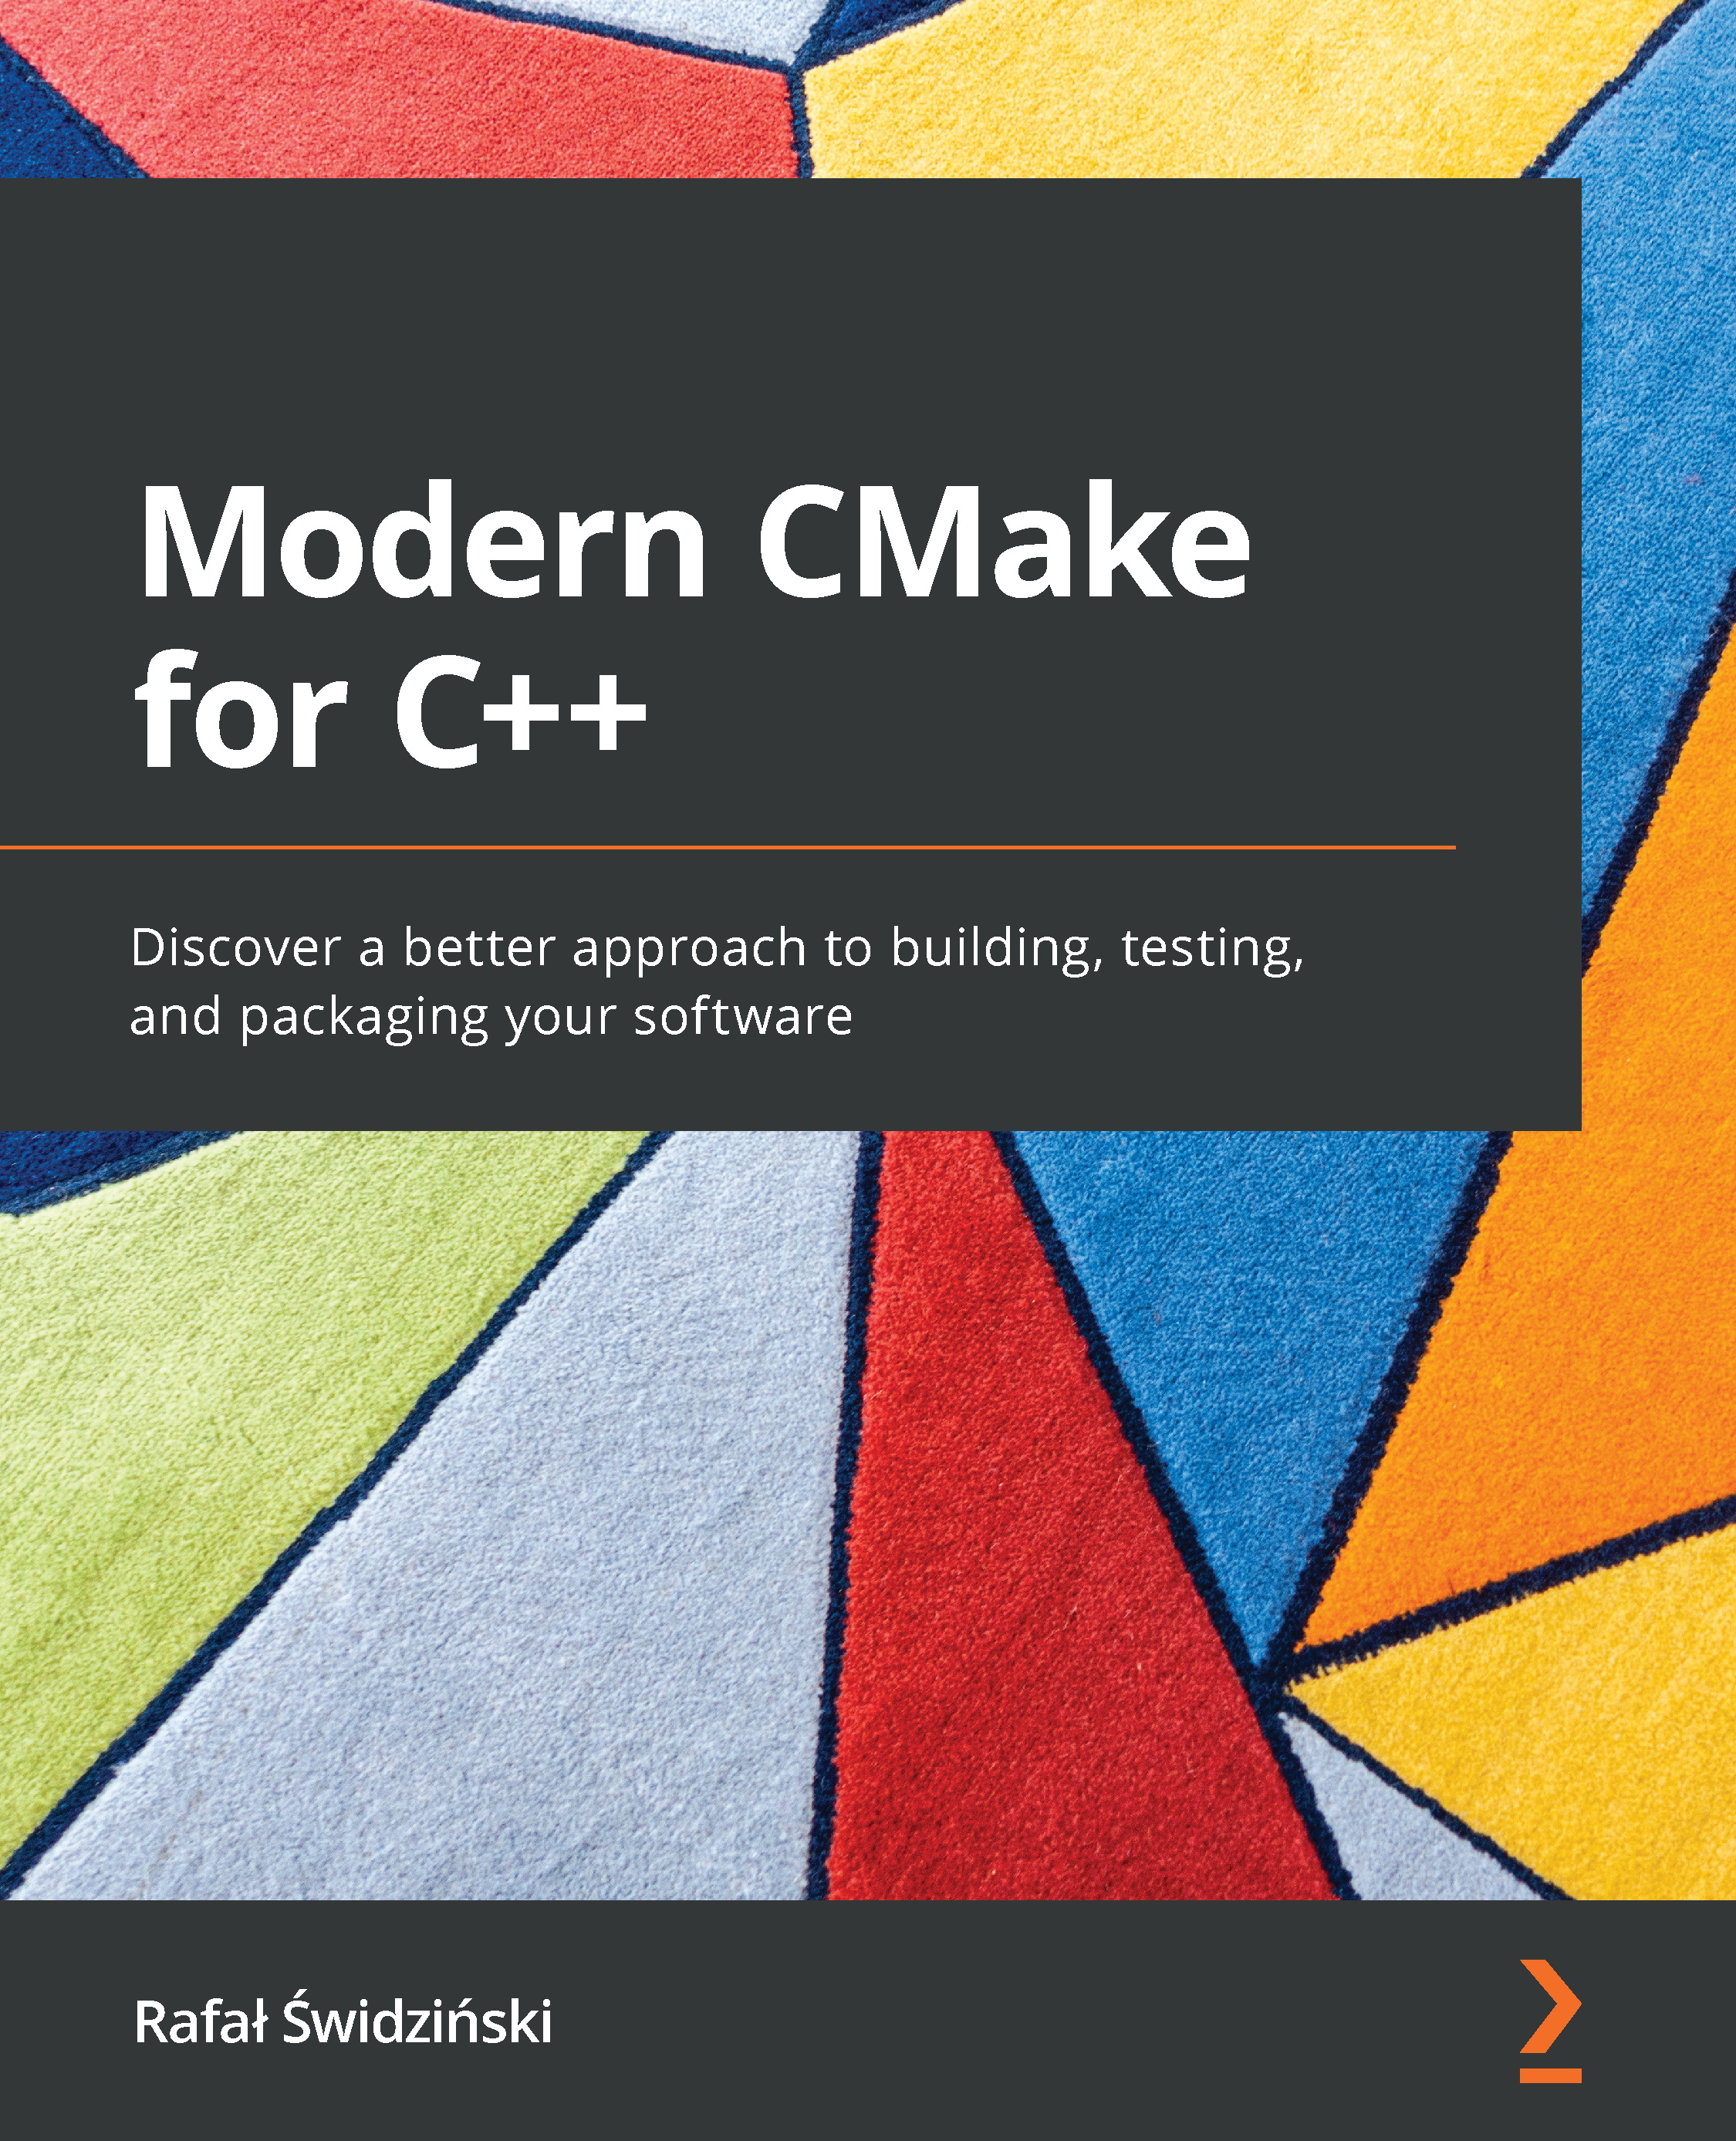
\includegraphics[width=\textwidth,height=\textheight,keepaspectratio]{cover.jpg}
		\begin{tikzpicture}[remember picture, overlay, inner sep=0pt]
			\node at (current page.center) 
			{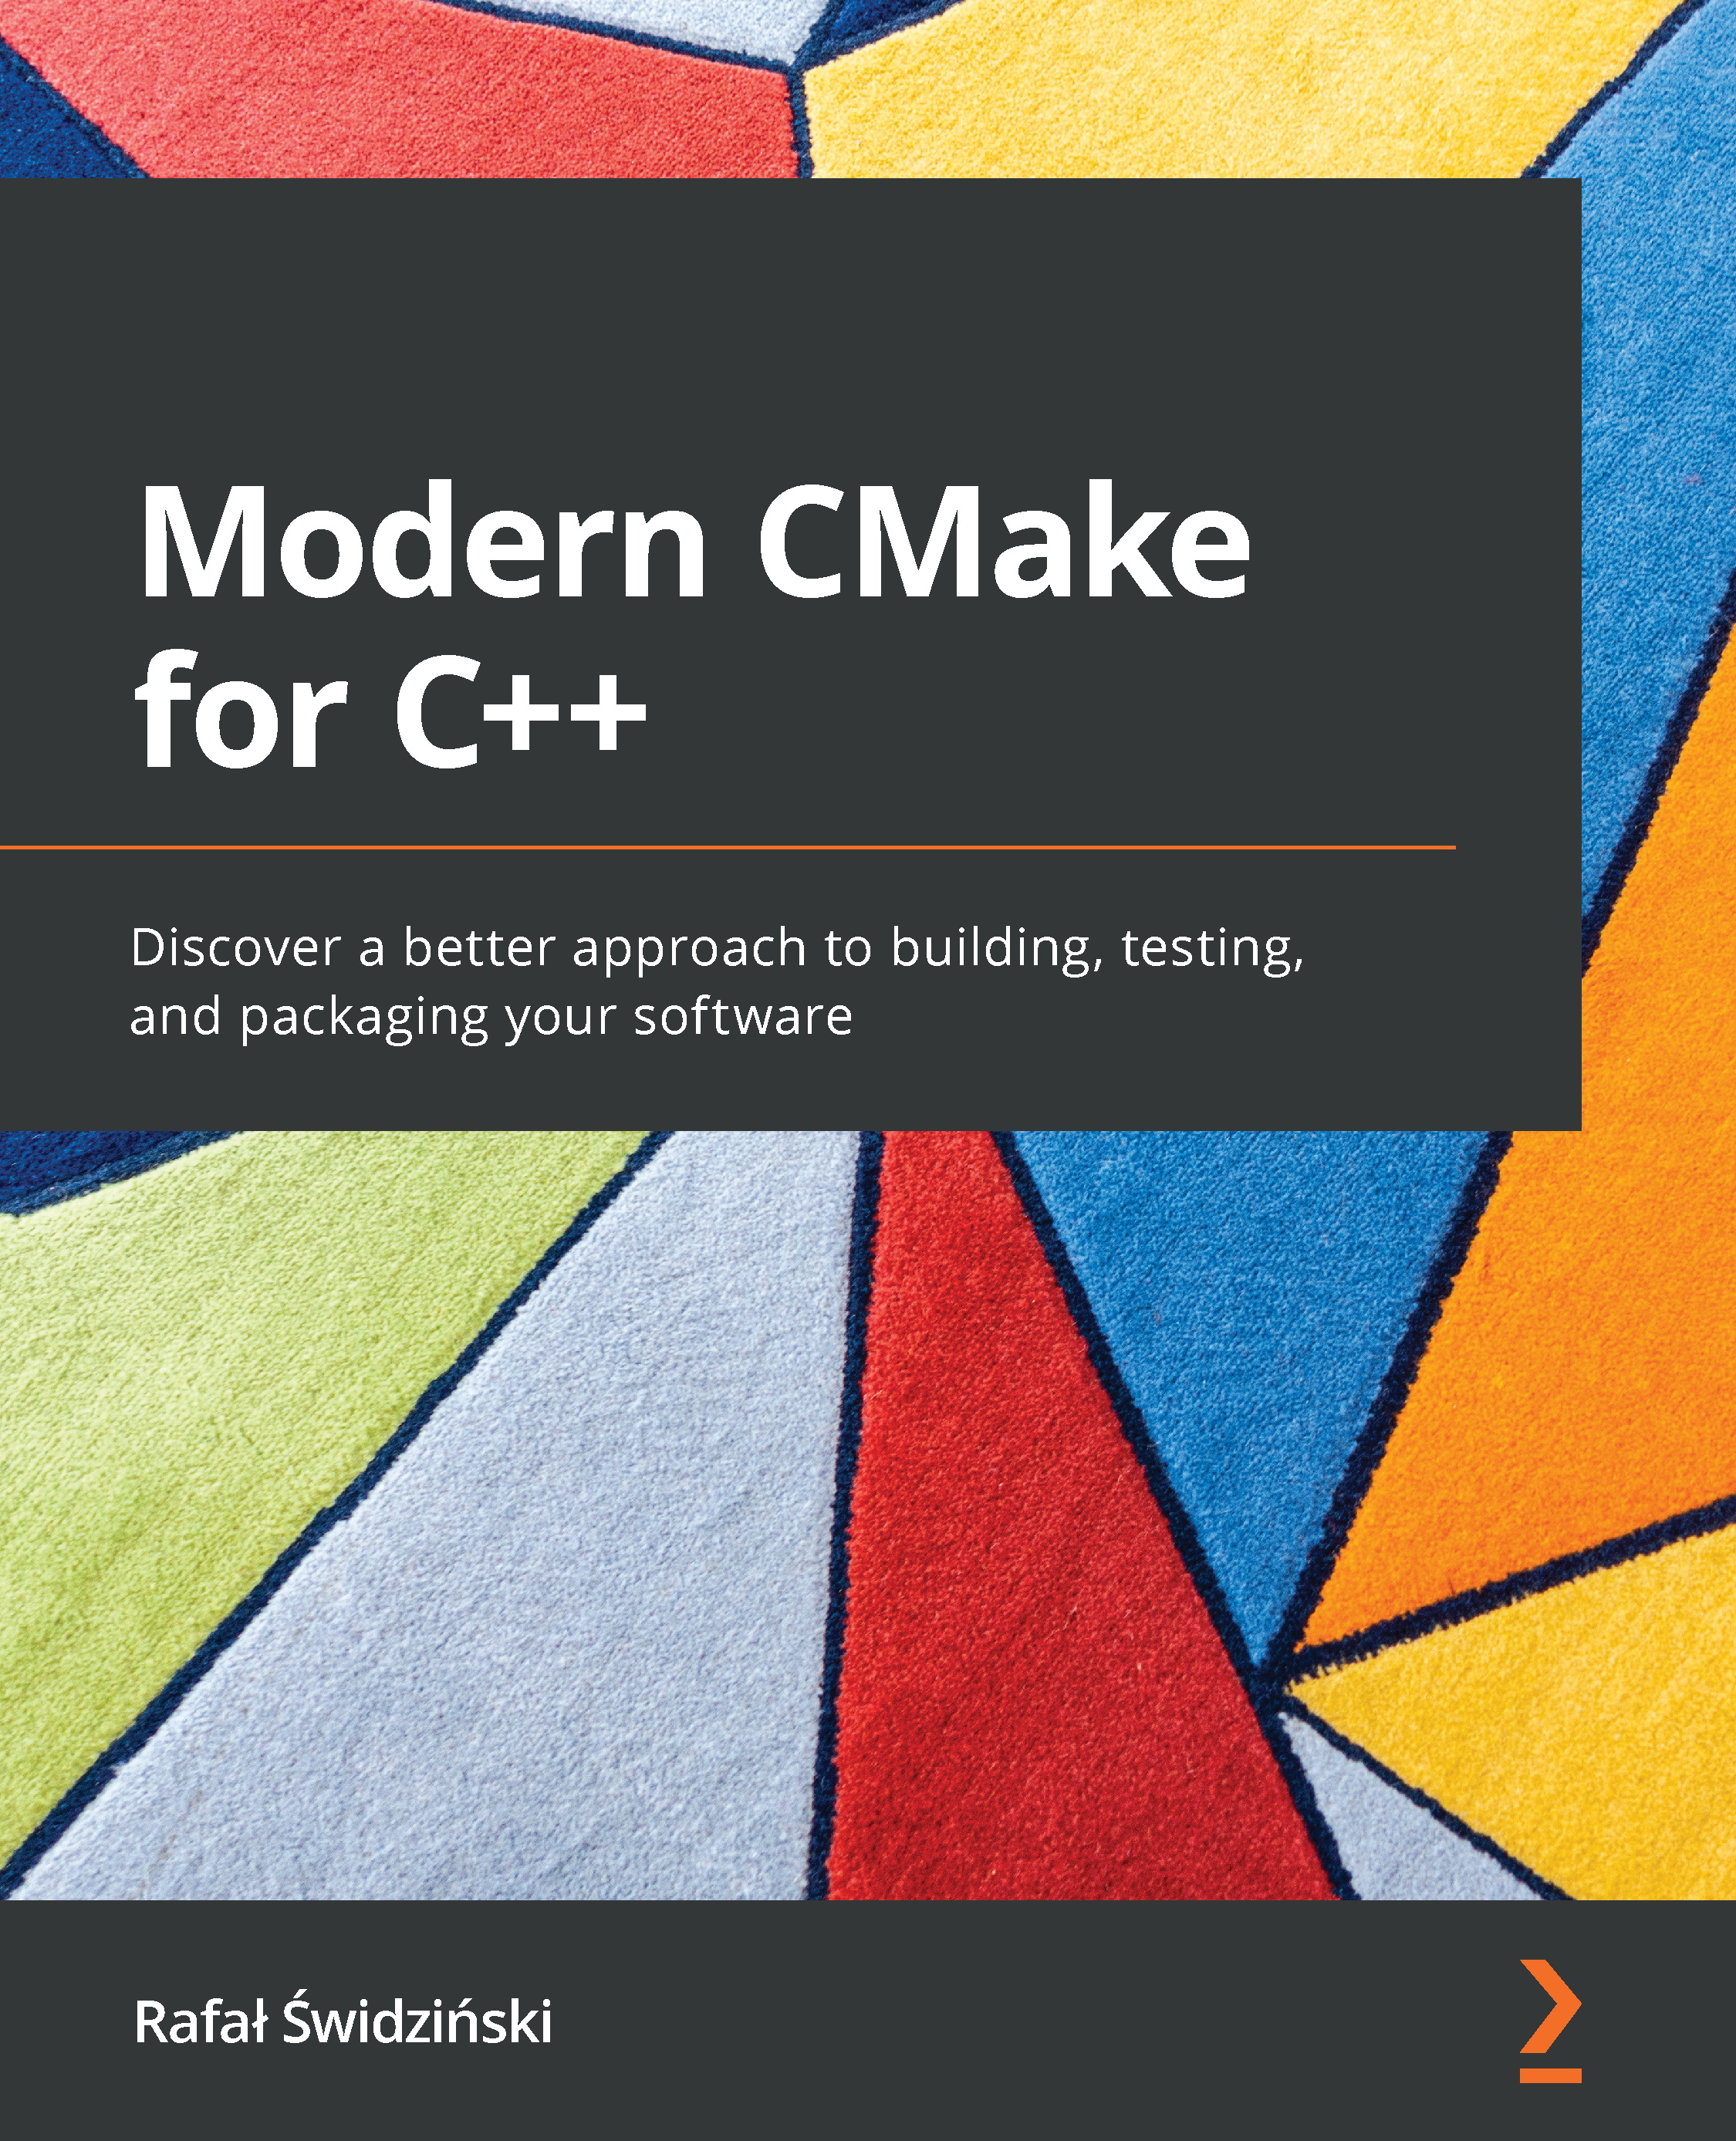
\includegraphics[width=\paperwidth, keepaspectratio=false]{cover.jpg}};
		\end{tikzpicture}
		\newpage
		\thispagestyle{empty}
		\huge
		\textbf{Modern CMake for C++} 
		\\[9pt]
		\normalsize
		Discover a better approach to building, testing, and packaging your software
		\\[9pt]
		\normalsize
		了解构建、测试和打包软件更好的方法
		\\[10pt]
		\normalsize 
		作者: Rafał Świdziński
		\\[8pt]
		\normalsize
		译者:陈晓伟
	\end{center}
	
	\hspace*{\fill} \\ %插入空行
	\noindent\textbf{本书概述}
	
	创建一流的软件是一项极其困难的任务。研究这一主题的开发人员很难确定哪些建议是最新的,哪些方法已经可以用更简单、更好的实践所取代。与此同时,大多数在线资源提供的解释有限,也缺乏适当的上下文和结构。
	
	本书提供了一种更简单、更全面的体验,全面地介绍了如何构建C+解决方案。Modern CMake for C++是一个端到端的复杂任务自动化指南,包括构建、测试和打包。您不仅将可以了解如何在CMake项目中使用CMake语言,还将发现是什么使它们可维护,优雅和干净。本书还关注源目录、构建目标和包的结构。随着深入的了解进展,您将学习如何编译和链接可执行文件和库,这些过程如何工作,以及如何优化CMake中的构建以获得最佳结果。您将了解如何在您的项目中使用外部依赖项——第三方库、测试框架、程序分析工具和文档生成器。最后,将掌握用于内部和外部目标的导出、安装和打包的技术。
	
	读完这本书,将能够自信地以专业的水平使用CMake。
	
	
	\hspace*{\fill} \\ %插入空行
	\noindent\textbf{关键特性}
	\begin{itemize}
		\item 理解并自动化CMake编译和链接
		\item 轻松管理内部和外部依赖关系
		\item 添加质量检查和测试作为构建的固定步骤
	\end{itemize}
	
	\hspace*{\fill} \\ %插入空行
	\noindent\textbf{作者简介}
	
	\textbf{Rafał Świdziński}在Google公司担任专职工程师。作为一名拥有超过10年专业经验的全栈开发人员,能够尝试大量的编程语言和技术。期间,他一直在自己的公司和包括Cisco Meraki、Amazon和Ericsson在内的公司开发软件。他来自波兰的罗兹(Łódź),现在住在英国伦敦,在那里他经营一个YouTube频道“Smok”,讨论与软件开发相关的话题。他很喜欢处理技术问题,包括许多人在该领域遇到挑战。在他的整个工作中,他详细解释了技术概念,并揭开了软件工程师角色背后的艺术和科学的神秘面纱。他的主要关注代码质量和编程技巧。
	
	\hspace*{\fill} \\ %插入空行
	\noindent\textbf{本书相关}
	\begin{itemize}
		\item Github地址:\\\url{https://github.com/xiaoweiChen/Modern-CMake-For-CXX}
	\end{itemize}
	\newpage
	
	%前言
	\pagestyle{empty}
	\subfile{content/preface.tex}
	\newpage
	
	\tableofcontents
	\newpage

	\setsecnumdepth{section}
	
	\color{white}
	\section*{\zihao{1}第一部分:基础知识}
	\pagecolor{mygray}
	\addcontentsline{toc}{section}{第一部分:基础知识}
	\textbf{\subfile{content/1/Section.tex}}
	\newpage
	\color{black}
	\pagecolor{white}

	\subsection*{\zihao{2} 第1章\hspace{0.5cm}初识CMake}
	\addcontentsline{toc}{subsection}{第1章\hspace{0.5cm}初识CMake}
	\subfile{content/1/chapter1/0.tex}
	
	\subsubsection*{\zihao{3} 1.1.\hspace{0.2cm}相关准备}
	\addcontentsline{toc}{subsubsection}{1.1.\hspace{0.2cm}相关准备}
	\subfile{content/1/chapter1/1.tex}
	
	\subsubsection*{\zihao{3} 1.2.\hspace{0.2cm}基础知识}
	\addcontentsline{toc}{subsubsection}{1.2.\hspace{0.2cm}基础知识}
	\subfile{content/1/chapter1/2.tex}
	
	\subsubsection*{\zihao{3} 1.3.\hspace{0.2cm}不同平台的安装}
	\addcontentsline{toc}{subsubsection}{1.3.\hspace{0.2cm}不同平台的安装}
	\subfile{content/1/chapter1/3.tex}
	
	\subsubsection*{\zihao{3} 1.4.\hspace{0.2cm}使用命令行}
	\addcontentsline{toc}{subsubsection}{1.4.\hspace{0.2cm}使用命令行}
	\subfile{content/1/chapter1/4.tex}
	
	\subsubsection*{\zihao{3} 1.5.\hspace{0.2cm}项目文件}
	\addcontentsline{toc}{subsubsection}{1.5.\hspace{0.2cm}项目文件}
	\subfile{content/1/chapter1/5.tex}
	
	\subsubsection*{\zihao{3} 1.6.\hspace{0.2cm}脚本和模块}
	\addcontentsline{toc}{subsubsection}{1.6.\hspace{0.2cm}脚本和模块}
	\subfile{content/1/chapter1/6.tex}
	
	\subsubsection*{\zihao{3} 1.7.\hspace{0.2cm}总结}
	\addcontentsline{toc}{subsubsection}{1.7.\hspace{0.2cm}总结}
	\subfile{content/1/chapter1/7.tex}
	
	\subsubsection*{\zihao{3} 1.8.\hspace{0.2cm}扩展阅读}
	\addcontentsline{toc}{subsubsection}{1.8.\hspace{0.2cm}扩展阅读}
	\subfile{content/1/chapter1/8.tex}
	\newpage
	
	\subsection*{\zihao{2} 第2章\hspace{0.5cm}CMake语法}
	\addcontentsline{toc}{subsection}{第2章\hspace{0.5cm}CMake语法}
	\subfile{content/1/chapter2/0.tex}
	
	\subsubsection*{\zihao{3} 2.1.\hspace{0.2cm}相关准备}
	\addcontentsline{toc}{subsubsection}{2.1.\hspace{0.2cm}相关准备}
	\subfile{content/1/chapter2/1.tex}
	
	\subsubsection*{\zihao{3} 2.2.\hspace{0.2cm}基本语法}
	\addcontentsline{toc}{subsubsection}{2.2.\hspace{0.2cm}基本语法}
	\subfile{content/1/chapter2/2.tex}
	
	\subsubsection*{\zihao{3} 2.3.\hspace{0.2cm}变量}
	\addcontentsline{toc}{subsubsection}{2.3.\hspace{0.2cm}变量}
	\subfile{content/1/chapter2/3.tex}
	
	\subsubsection*{\zihao{3} 2.4.\hspace{0.2cm}列表}
	\addcontentsline{toc}{subsubsection}{2.4.\hspace{0.2cm}列表}
	\subfile{content/1/chapter2/4.tex}
	
	\subsubsection*{\zihao{3} 2.5.\hspace{0.2cm}控制结构}
	\addcontentsline{toc}{subsubsection}{2.5.\hspace{0.2cm}控制结构}
	\subfile{content/1/chapter2/5.tex}
	
	\subsubsection*{\zihao{3} 2.6.\hspace{0.2cm}实用指令}
	\addcontentsline{toc}{subsubsection}{2.6.\hspace{0.2cm}实用指令}
	\subfile{content/1/chapter2/6.tex}
	
	\subsubsection*{\zihao{3} 2.7.\hspace{0.2cm}总结}
	\addcontentsline{toc}{subsubsection}{2.7.\hspace{0.2cm}总结}
	\subfile{content/1/chapter2/7.tex}
	
	\subsubsection*{\zihao{3} 2.8.\hspace{0.2cm}扩展阅读}
	\addcontentsline{toc}{subsubsection}{2.8.\hspace{0.2cm}扩展阅读}
	\subfile{content/1/chapter2/8.tex}
	\newpage
	
	\subsection*{\zihao{2} 第3章\hspace{0.5cm}CMake项目}
	\addcontentsline{toc}{subsection}{第3章\hspace{0.5cm}CMake项目}
	\subfile{content/1/chapter3/0.tex}
	
	\subsubsection*{\zihao{3} 3.1.\hspace{0.2cm}相关准备}
	\addcontentsline{toc}{subsubsection}{3.1.\hspace{0.2cm}相关准备}
	\subfile{content/1/chapter3/1.tex}
	
	\subsubsection*{\zihao{3} 3.2.\hspace{0.2cm}指令和命令}
	\addcontentsline{toc}{subsubsection}{3.2.\hspace{0.2cm}指令和命令}
	\subfile{content/1/chapter3/2.tex}
	
	\subsubsection*{\zihao{3} 3.3.\hspace{0.2cm}划分项目}
	\addcontentsline{toc}{subsubsection}{3.3.\hspace{0.2cm}划分项目}
	\subfile{content/1/chapter3/3.tex}
	
	\subsubsection*{\zihao{3} 3.4.\hspace{0.2cm}项目结构}
	\addcontentsline{toc}{subsubsection}{3.4.\hspace{0.2cm}项目结构}
	\subfile{content/1/chapter3/4.tex}
	
	\subsubsection*{\zihao{3} 3.5.\hspace{0.2cm}环境范围}
	\addcontentsline{toc}{subsubsection}{3.5.\hspace{0.2cm}环境范围}
	\subfile{content/1/chapter3/5.tex}
	
	\subsubsection*{\zihao{3} 3.6.\hspace{0.2cm}配置工具链}
	\addcontentsline{toc}{subsubsection}{3.6.\hspace{0.2cm}配置工具链}
	\subfile{content/1/chapter3/6.tex}
	
	\subsubsection*{\zihao{3} 3.7.\hspace{0.2cm}禁用内构建}
	\addcontentsline{toc}{subsubsection}{3.7.\hspace{0.2cm}禁用内构建}
	\subfile{content/1/chapter3/7.tex}
	
	\subsubsection*{\zihao{3} 3.8.\hspace{0.2cm}总结}
	\addcontentsline{toc}{subsubsection}{3.8.\hspace{0.2cm}总结}
	\subfile{content/1/chapter3/8.tex}
	
	\subsubsection*{\zihao{3} 3.9.\hspace{0.2cm}扩展阅读}
	\addcontentsline{toc}{subsubsection}{3.9.\hspace{0.2cm}扩展阅读}
	\subfile{content/1/chapter3/9.tex}
	\newpage
	
	\color{white}
	\section*{\zihao{1}第二部分:进行构建}
	\pagecolor{mygray}
	\addcontentsline{toc}{section}{第二部分:进行构建}
	\textbf{\subfile{content/2/Section.tex}}
	\newpage
	\color{black}
	\pagecolor{white}
	
	\subsection*{\zihao{2} 第4章\hspace{0.5cm}使用目标}
	\addcontentsline{toc}{subsection}{第4章\hspace{0.5cm}使用目标}
	\subfile{content/2/chapter4/0.tex}
	
	\subsubsection*{\zihao{3} 4.1.\hspace{0.2cm}相关准备}
	\addcontentsline{toc}{subsubsection}{4.1.\hspace{0.2cm}相关准备}
	\subfile{content/2/chapter4/1.tex}
	
	\subsubsection*{\zihao{3} 4.2.\hspace{0.2cm}目标的概念}
	\addcontentsline{toc}{subsubsection}{4.2.\hspace{0.2cm}目标的概念}
	\subfile{content/2/chapter4/2.tex}
	
	\subsubsection*{\zihao{3} 4.3.\hspace{0.2cm}编写自定义命令}
	\addcontentsline{toc}{subsubsection}{4.3.\hspace{0.2cm}编写自定义命令}
	\subfile{content/2/chapter4/3.tex}
	
	\subsubsection*{\zihao{3} 4.4.\hspace{0.2cm}生成器表达式}
	\addcontentsline{toc}{subsubsection}{4.4.\hspace{0.2cm}生成器表达式}
	\subfile{content/2/chapter4/4.tex}
	
	\subsubsection*{\zihao{3} 4.5.\hspace{0.2cm}总结}
	\addcontentsline{toc}{subsubsection}{4.5.\hspace{0.2cm}总结}
	\subfile{content/2/chapter4/5.tex}
	\newpage
	
	\subsection*{\zihao{2} 第5章\hspace{0.5cm}CMake编译C++}
	\addcontentsline{toc}{subsection}{第5章\hspace{0.5cm}CMake编译C++}
	\subfile{content/2/chapter5/0.tex}
	
	\subsubsection*{\zihao{3} 5.1.\hspace{0.2cm}相关准备}
	\addcontentsline{toc}{subsubsection}{5.1.\hspace{0.2cm}相关准备}
	\subfile{content/2/chapter5/1.tex}
	
	\subsubsection*{\zihao{3} 5.2.\hspace{0.2cm}编译基础}
	\addcontentsline{toc}{subsubsection}{5.2.\hspace{0.2cm}编译基础}
	\subfile{content/2/chapter5/2.tex}
	
	\subsubsection*{\zihao{3} 5.3.\hspace{0.2cm}预处理配置}
	\addcontentsline{toc}{subsubsection}{5.3.\hspace{0.2cm}预处理配置}
	\subfile{content/2/chapter5/3.tex}
	
	\subsubsection*{\zihao{3} 5.4.\hspace{0.2cm}配置优化器}
	\addcontentsline{toc}{subsubsection}{5.4.\hspace{0.2cm}配置优化器}
	\subfile{content/2/chapter5/4.tex}
	
	\subsubsection*{\zihao{3} 5.5.\hspace{0.2cm}编译过程}
	\addcontentsline{toc}{subsubsection}{5.5.\hspace{0.2cm}编译过程}
	\subfile{content/2/chapter5/5.tex}
	
	\subsubsection*{\zihao{3} 5.6.\hspace{0.2cm}总结}
	\addcontentsline{toc}{subsubsection}{5.6.\hspace{0.2cm}总结}
	\subfile{content/2/chapter5/6.tex}
	\newpage
	
	\subsection*{\zihao{2} 第6章\hspace{0.5cm}进行链接}
	\addcontentsline{toc}{subsection}{第6章\hspace{0.5cm}进行链接}
	\subfile{content/2/chapter6/0.tex}
	
	\subsubsection*{\zihao{3} 6.1.\hspace{0.2cm}相关准备}
	\addcontentsline{toc}{subsubsection}{6.1.\hspace{0.2cm}相关准备}
	\subfile{content/2/chapter6/1.tex}
	
	\subsubsection*{\zihao{3} 6.2.\hspace{0.2cm}掌握正确的链接方式}
	\addcontentsline{toc}{subsubsection}{6.2.\hspace{0.2cm}掌握正确的链接方式}
	\subfile{content/2/chapter6/2.tex}
	
	\subsubsection*{\zihao{3} 6.3.\hspace{0.2cm}构建不同类型的库}
	\addcontentsline{toc}{subsubsection}{6.3.\hspace{0.2cm}构建不同类型的库}
	\subfile{content/2/chapter6/3.tex}
	
	\subsubsection*{\zihao{3} 6.4.\hspace{0.2cm}用定义规则解决问题}
	\addcontentsline{toc}{subsubsection}{6.4.\hspace{0.2cm}用定义规则解决问题}
	\subfile{content/2/chapter6/4.tex}
	
	\subsubsection*{\zihao{3} 6.5.\hspace{0.2cm}连接顺序和未定义符号}
	\addcontentsline{toc}{subsubsection}{6.5.\hspace{0.2cm}连接顺序和未定义符号}
	\subfile{content/2/chapter6/5.tex}
	
	\subsubsection*{\zihao{3} 6.6.\hspace{0.2cm}分离main()进行测试}
	\addcontentsline{toc}{subsubsection}{6.6.\hspace{0.2cm}分离main()进行测试}
	\subfile{content/2/chapter6/6.tex}
	
	\subsubsection*{\zihao{3} 6.7.\hspace{0.2cm}总结}
	\addcontentsline{toc}{subsubsection}{6.7.\hspace{0.2cm}总结}
	\subfile{content/2/chapter6/7.tex}
	
	\subsubsection*{\zihao{3} 6.8.\hspace{0.2cm}扩展阅读}
	\addcontentsline{toc}{subsubsection}{6.8.\hspace{0.2cm}扩展阅读}
	\subfile{content/2/chapter6/8.tex}
	\newpage
	
	\subsection*{\zihao{2} 第7章\hspace{0.5cm}管理依赖关系}
	\addcontentsline{toc}{subsection}{第7章\hspace{0.5cm}管理依赖关系}
	\subfile{content/2/chapter7/0.tex}
	
	\subsubsection*{\zihao{3} 7.1.\hspace{0.2cm}相关准备}
	\addcontentsline{toc}{subsubsection}{7.1.\hspace{0.2cm}相关准备}
	\subfile{content/2/chapter7/1.tex}
	
	\subsubsection*{\zihao{3} 7.2.\hspace{0.2cm}如何查找已安装的软件包}
	\addcontentsline{toc}{subsubsection}{7.2.\hspace{0.2cm}如何查找已安装的软件包}
	\subfile{content/2/chapter7/2.tex}
	
	\subsubsection*{\zihao{3} 7.3.\hspace{0.2cm}使用FindPkgConfig0发现遗留包}
	\addcontentsline{toc}{subsubsection}{7.3.\hspace{0.2cm}使用FindPkgConfig0发现遗留包}
	\subfile{content/2/chapter7/3.tex}
	
	\subsubsection*{\zihao{3} 7.4.\hspace{0.2cm}编写自己的查找模块}
	\addcontentsline{toc}{subsubsection}{7.4.\hspace{0.2cm}编写自己的查找模块}
	\subfile{content/2/chapter7/4.tex}
	
	\subsubsection*{\zihao{3} 7.5.\hspace{0.2cm}使用Git库}
	\addcontentsline{toc}{subsubsection}{7.5.\hspace{0.2cm}使用Git库}
	\subfile{content/2/chapter7/5.tex}
	
	\subsubsection*{\zihao{3} 7.6.\hspace{0.2cm}使用ExternalProject和FetchContent模块}
	\addcontentsline{toc}{subsubsection}{7.6.\hspace{0.2cm}使用ExternalProject和FetchContent模块}
	\subfile{content/2/chapter7/6.tex}
	
	\subsubsection*{\zihao{3} 7.7.\hspace{0.2cm}总结}
	\addcontentsline{toc}{subsubsection}{7.7.\hspace{0.2cm}总结}
	\subfile{content/2/chapter7/7.tex}
	
	\subsubsection*{\zihao{3} 7.8.\hspace{0.2cm}扩展阅读}
	\addcontentsline{toc}{subsubsection}{7.8.\hspace{0.2cm}扩展阅读}
	\subfile{content/2/chapter7/8.tex}
	\newpage
	
	\color{white}
	\section*{\zihao{1}第三部分:自动化}
	\pagecolor{mygray}
	\addcontentsline{toc}{section}{第三部分:自动化}
	\textbf{\subfile{content/3/Section.tex}}
	\newpage
	\color{black}
	\pagecolor{white}
	\newpage
	
	\subsection*{\zihao{2} 第8章\hspace{0.5cm}测试框架}
	\addcontentsline{toc}{subsection}{第8章\hspace{0.5cm}测试框架}
	\subfile{content/3/chapter8/0.tex}
	
	\subsubsection*{\zihao{3} 8.1.\hspace{0.2cm}相关准备}
	\addcontentsline{toc}{subsubsection}{8.1.\hspace{0.2cm}相关准备}
	\subfile{content/3/chapter8/1.tex}
	
	\subsubsection*{\zihao{3} 8.2.\hspace{0.2cm}为什么自动化测试值得这么麻烦?}
	\addcontentsline{toc}{subsubsection}{8.2.\hspace{0.2cm}为什么自动化测试值得这么麻烦?}
	\subfile{content/3/chapter8/2.tex}
	
	\subsubsection*{\zihao{3} 8.3.\hspace{0.2cm}使用CTest来标准化CMake中的测试}
	\addcontentsline{toc}{subsubsection}{8.3.\hspace{0.2cm}使用CTest来标准化CMake中的测试}
	\subfile{content/3/chapter8/3.tex}
	
	\subsubsection*{\zihao{3} 8.4.\hspace{0.2cm}为CTest创建最基本的单元测试}
	\addcontentsline{toc}{subsubsection}{8.4.\hspace{0.2cm}为CTest创建最基本的单元测试}
	\subfile{content/3/chapter8/4.tex}
	
	\subsubsection*{\zihao{3} 8.5.\hspace{0.2cm}单元测试框架}
	\addcontentsline{toc}{subsubsection}{8.5.\hspace{0.2cm}单元测试框架}
	\subfile{content/3/chapter8/5.tex}
	
	\subsubsection*{\zihao{3} 8.6.\hspace{0.2cm}生成测试覆盖报告}
	\addcontentsline{toc}{subsubsection}{8.6.\hspace{0.2cm}生成测试覆盖报告}
	\subfile{content/3/chapter8/6.tex}
	
	\subsubsection*{\zihao{3} 8.7.\hspace{0.2cm}总结}
	\addcontentsline{toc}{subsubsection}{8.7.\hspace{0.2cm}总结}
	\subfile{content/3/chapter8/7.tex}
	
	\subsubsection*{\zihao{3} 8.8.\hspace{0.2cm}扩展阅读}
	\addcontentsline{toc}{subsubsection}{8.8.\hspace{0.2cm}扩展阅读}
	\subfile{content/3/chapter8/8.tex}
	\newpage
	
	\subsection*{\zihao{2} 第9章\hspace{0.5cm}分析工具}
	\addcontentsline{toc}{subsection}{第9章\hspace{0.5cm}分析工具}
	\subfile{content/3/chapter9/0.tex}
	
	\subsubsection*{\zihao{3} 9.1.\hspace{0.2cm}相关准备}
	\addcontentsline{toc}{subsubsection}{9.1.\hspace{0.2cm}相关准备}
	\subfile{content/3/chapter9/1.tex}
	
	\subsubsection*{\zihao{3} 9.2.\hspace{0.2cm}格式化}
	\addcontentsline{toc}{subsubsection}{9.2.\hspace{0.2cm}格式化}
	\subfile{content/3/chapter9/2.tex}
	
	\subsubsection*{\zihao{3} 9.3.\hspace{0.2cm}静态检查}
	\addcontentsline{toc}{subsubsection}{9.3.\hspace{0.2cm}静态检查}	
	\subfile{content/3/chapter9/3.tex}
	
	\subsubsection*{\zihao{3} 9.4.\hspace{0.2cm}Valgrind的动态分析}
	\addcontentsline{toc}{subsubsection}{9.4.\hspace{0.2cm}Valgrind的动态分析}
	\subfile{content/3/chapter9/4.tex}
	
	\subsubsection*{\zihao{3} 9.5.\hspace{0.2cm}总结}
	\addcontentsline{toc}{subsubsection}{9.5.\hspace{0.2cm}总结}
	\subfile{content/3/chapter9/5.tex}
	
	\subsubsection*{\zihao{3} 9.6.\hspace{0.2cm}扩展阅读}
	\addcontentsline{toc}{subsubsection}{9.6.\hspace{0.2cm}扩展阅读}
	\subfile{content/3/chapter9/6.tex}
	\newpage
	
	\subsection*{\zihao{2} 第10章\hspace{0.5cm}生成文档}
	\addcontentsline{toc}{subsection}{第10章\hspace{0.5cm}生成文档}
	\subfile{content/3/chapter10/0.tex}
	
	\subsubsection*{\zihao{3} 10.1.\hspace{0.2cm}相关准备}
	\addcontentsline{toc}{subsubsection}{10.1.\hspace{0.2cm}相关准备}
	\subfile{content/3/chapter10/1.tex}
	
	\subsubsection*{\zihao{3} 10.2.\hspace{0.2cm}添加Doxygen}
	\addcontentsline{toc}{subsubsection}{10.2.\hspace{0.2cm}添加Doxygen}
	\subfile{content/3/chapter10/2.tex}
	
	\subsubsection*{\zihao{3} 10.3.\hspace{0.2cm}生成好看的文档}
	\addcontentsline{toc}{subsubsection}{10.3.\hspace{0.2cm}生成好看的文档}
	\subfile{content/3/chapter10/3.tex}
	
	\subsubsection*{\zihao{3} 10.4.\hspace{0.2cm}总结}
	\addcontentsline{toc}{subsubsection}{10.4.\hspace{0.2cm}总结}
	\subfile{content/3/chapter10/4.tex}
	
	\subsubsection*{\zihao{3} 10.5.\hspace{0.2cm}扩展阅读}
	\addcontentsline{toc}{subsubsection}{10.5.\hspace{0.2cm}扩展阅读}
	\subfile{content/3/chapter10/5.tex}
	\newpage
	
	\subsection*{\zihao{2} 第11章\hspace{0.5cm}安装和打包}
	\addcontentsline{toc}{subsection}{第11章\hspace{0.5cm}安装和打包}
	\subfile{content/3/chapter11/0.tex}
	
	\subsubsection*{\zihao{3} 11.1.\hspace{0.2cm}相关准备}
	\addcontentsline{toc}{subsubsection}{11.1.\hspace{0.2cm}相关准备}
	\subfile{content/3/chapter11/1.tex}
	
	\subsubsection*{\zihao{3} 11.2.\hspace{0.2cm}只导出,不安装}
	\addcontentsline{toc}{subsubsection}{11.2.\hspace{0.2cm}只导出,不安装}
	\subfile{content/3/chapter11/2.tex}
	
	\subsubsection*{\zihao{3} 11.3.\hspace{0.2cm}在系统上安装}
	\addcontentsline{toc}{subsubsection}{11.3.\hspace{0.2cm}在系统上安装}
	\subfile{content/3/chapter11/3.tex}
	
	\subsubsection*{\zihao{3} 11.4.\hspace{0.2cm}创建可重用的包}
	\addcontentsline{toc}{subsubsection}{11.4.\hspace{0.2cm}创建可重用的包}
	\subfile{content/3/chapter11/4.tex}
	
	\subsubsection*{\zihao{3} 11.5.\hspace{0.2cm}定义组件}
	\addcontentsline{toc}{subsubsection}{11.5.\hspace{0.2cm}定义组件}
	\subfile{content/3/chapter11/5.tex}
	
	\subsubsection*{\zihao{3} 11.6.\hspace{0.2cm}使用CPack打包}
	\addcontentsline{toc}{subsubsection}{11.6.\hspace{0.2cm}使用CPack打包}
	\subfile{content/3/chapter11/6.tex}
	
	\subsubsection*{\zihao{3} 11.7.\hspace{0.2cm}总结}
	\addcontentsline{toc}{subsubsection}{11.7.\hspace{0.2cm}总结}
	\subfile{content/3/chapter11/7.tex}
	
	\subsubsection*{\zihao{3} 11.8.\hspace{0.2cm}扩展阅读}
	\addcontentsline{toc}{subsubsection}{11.8.\hspace{0.2cm}扩展阅读}
	\subfile{content/3/chapter11/8.tex}
	\newpage
	
	\subsection*{\zihao{2} 第12章\hspace{0.5cm}创建完整的项目}
	\addcontentsline{toc}{subsection}{第12章\hspace{0.5cm}创建完整的项目}
	\subfile{content/3/chapter12/0.tex}
	
	\subsubsection*{\zihao{3} 12.1.\hspace{0.2cm}相关准备}
	\addcontentsline{toc}{subsubsection}{12.1.\hspace{0.2cm}相关准备}
	\subfile{content/3/chapter12/1.tex}
	
	\subsubsection*{\zihao{3} 12.2.\hspace{0.2cm}Planning our work}
	\addcontentsline{toc}{subsubsection}{12.2.\hspace{0.2cm}Planning our work}
	\subfile{content/3/chapter12/2.tex}
	
	\subsubsection*{\zihao{3} 12.3.\hspace{0.2cm}Project layout}
	\addcontentsline{toc}{subsubsection}{12.3.\hspace{0.2cm}Project layout}
	\subfile{content/3/chapter12/3.tex}
	
	\subsubsection*{\zihao{3} 12.4.\hspace{0.2cm}Building and managing dependencies}
	\addcontentsline{toc}{subsubsection}{12.4.\hspace{0.2cm}Building and managing dependencies}
	\subfile{content/3/chapter12/4.tex}
	
	\subsubsection*{\zihao{3} 12.5.\hspace{0.2cm}Testing and program analysis}
	\addcontentsline{toc}{subsubsection}{12.5.\hspace{0.2cm}Testing and program analysis}
	\subfile{content/3/chapter12/5.tex}
	
	\subsubsection*{\zihao{3} 12.6.\hspace{0.2cm}Installing and packaging}
	\addcontentsline{toc}{subsubsection}{12.6.\hspace{0.2cm}Installing and packaging}
	\subfile{content/3/chapter12/6.tex}
	
	\subsubsection*{\zihao{3} 12.7.\hspace{0.2cm}Providing the documentation}
	\addcontentsline{toc}{subsubsection}{12.7.\hspace{0.2cm}Providing the documentation}
	\subfile{content/3/chapter12/7.tex}
	
	\subsubsection*{\zihao{3} 12.8.\hspace{0.2cm}总结}
	\addcontentsline{toc}{subsubsection}{12.8.\hspace{0.2cm}总结}
	\subfile{content/3/chapter12/8.tex}
	
	\subsubsection*{\zihao{3} 12.9.\hspace{0.2cm}扩展阅读}
	\addcontentsline{toc}{subsubsection}{12.9.\hspace{0.2cm}扩展阅读}
	\subfile{content/3/chapter12/9.tex}
	\newpage
	
	\section*{\zihao{2} 附录:其它指令}
	\addcontentsline{toc}{section}{附录:其它指令}
	\subfile{content/Appendix/0.tex}
	
	\subsubsection*{\zihao{3}string()指令}
	\addcontentsline{toc}{subsubsection}{string()指令}
	\subfile{content/Appendix/1.tex}
	
	\subsubsection*{\zihao{3}list()指令}
	\addcontentsline{toc}{subsubsection}{list()指令}
	\subfile{content/Appendix/2.tex}
	
	\subsubsection*{\zihao{3}file()指令}
	\addcontentsline{toc}{subsubsection}{file()指令}
	\subfile{content/Appendix/3.tex}
	
	\subsubsection*{\zihao{3}math()指令}
	\addcontentsline{toc}{subsubsection}{math()指令}
	\subfile{content/Appendix/4.tex}
	\newpage

\end{sloppypar}
\end{document}

